% to choose your degree
% please un-comment just one of the following

\documentclass[bsc,frontabs,twoside,singlespacing,parskip,deptreport,logo]{infthesis}     % for BSc, BEng etc.
% \documentclass[minf,frontabs,twoside,singlespacing,parskip,deptreport]{infthesis}  % for MInf


\usepackage{tikz}
\usetikzlibrary{timeline}


\usepackage{graphicx}
\usepackage{url}
\usepackage{amsmath}
\usepackage{caption}
\usepackage{subcaption}
\usepackage{gensymb}
\usepackage[capposition=bottom]{floatrow}


\graphicspath{ {Pictures/background/}{Pictures/models/}{Pictures/elastica/}{Pictures/illusions/}{Pictures/experiments/rnn/} {Pictures/experiments/exp1_fig2/} {Pictures/experiments/fig5/} {Pictures/experiments/fig5/figB}}



\newcommand{\plottwofigures}[4]{
\begin{figure}[H]
\centering
\begin{subfigure}{.5\textwidth}
  \caption{}
  \centering
  \includegraphics[width=.8\linewidth]{#1}
\end{subfigure}%
\begin{subfigure}{.5\textwidth}
  \caption{}
  \centering
  \includegraphics[width=.8\linewidth]{#2}
\end{subfigure}
\caption[#4]{#3}
\label{#1}
\end{figure}
}


\newcommand{\plottwofiguresS}[5]{
\begin{figure}[H]
\centering
\begin{subfigure}{.5\textwidth}
  \caption{}
  \centering
  \includegraphics[width=#5\linewidth]{#1}
\end{subfigure}%
\begin{subfigure}{.5\textwidth}
  \caption{}
  \centering
  \includegraphics[width=#5\linewidth]{#2}
\end{subfigure}
\caption[#4]{#3}
\label{#1}
\end{figure}
}


\newcommand{\plotfigure}[3]{
\begin{figure}[H]
\centering
\includegraphics[width=.8\linewidth]{#1}
\caption[#3]{#2}
\label{#1}
\end{figure}
}


\newcommand{\plotfigureS}[4]{
\begin{figure}[H]
\centering
\includegraphics[width=#4\linewidth]{#1}
\caption[#3]{#2}
\label{#1}
\end{figure}
}

\newcommand{\plotthreefigures}[6]{
\begin{figure}[H]
\begin{subfigure}{.33\textwidth}
  \centering
  \includegraphics[width=#6\linewidth]{#1}
  \caption{}
\end{subfigure}%
\hfill
\begin{subfigure}{.33\textwidth}
  \centering
  \includegraphics[width=#6\linewidth]{#2}
  \caption{}
\end{subfigure}
\hfill
\begin{subfigure}{.33\textwidth}
  \centering
  \includegraphics[width=#6\linewidth]{#3}
  \caption{}
\end{subfigure}%
\label{#1}
\caption[#5]{#4}
\end{figure}
}

\newcommand{\plotfigures}[5]{
\begin{figure}[H]
\caption{}
\begin{subfigure}{.5\textwidth}
  \caption{}
  \centering
  \includegraphics[width=1\linewidth]{#1}
\end{subfigure}%
\begin{subfigure}{.5\textwidth}
  \caption{}
  \centering
  \includegraphics[width=1\linewidth]{#2}
\end{subfigure}
\begin{subfigure}{.5\textwidth}
  \caption{}
  \centering
  \includegraphics[width=1\linewidth]{#3}
\end{subfigure}%
\begin{subfigure}{.5\textwidth}
  \caption{}
  \centering
  \includegraphics[width=.1\linewidth]{#4}
\end{subfigure}
\label{#1}
\floatfoot{#5}
\end{figure}
}

\newcommand{\plotfiguresix}[9]{
\begin{figure}[H]
\centering
\begin{subfigure}[b]{#8\textwidth}
  \centering
  \includegraphics[width=\textwidth]{#1}
  \caption{}
\end{subfigure}
\hfill
\begin{subfigure}[b]{#8\textwidth}
  \centering
  \includegraphics[width=\textwidth]{#2}
  \caption{}
\end{subfigure}
\hfill
\begin{subfigure}[b]{#8\textwidth}
  \centering
  \includegraphics[width=\textwidth]{#3}
  \caption{}
\end{subfigure}
\hfill
\begin{subfigure}[b]{#8\textwidth}
  \centering
  \includegraphics[width=\textwidth]{#4}
  \caption{}
\end{subfigure}
\hfill
\begin{subfigure}[b]{#8\textwidth}
  \centering
  \includegraphics[width=\textwidth]{#5}
  \caption{}
\end{subfigure}
\hfill
\begin{subfigure}[b]{#8\textwidth}
  \centering
  \includegraphics[width=\textwidth]{#6}
  \caption{}
\end{subfigure}
\caption[#9]{#7}
\label{#1}
\end{figure}
}

\newcommand{\plotfiguresixn}[7]{
\begin{figure}[H]
\caption{}
\begin{subfigure}{.5\textwidth}
  \centering
  \includegraphics[width=.8\linewidth]{#1}
\end{subfigure}%
\begin{subfigure}{.5\textwidth}
  \centering
  \includegraphics[width=.8\linewidth]{#2}
\end{subfigure}
\begin{subfigure}{.5\textwidth}
  \centering
  \includegraphics[width=.8\linewidth]{#3}
\end{subfigure}%
\begin{subfigure}{.5\textwidth}
  \centering
  \includegraphics[width=.8\linewidth]{#4}
\end{subfigure}
\begin{subfigure}{.5\textwidth}
  \centering
  \includegraphics[width=.8\linewidth]{#5}
\end{subfigure}%
\begin{subfigure}{.5\textwidth}
  \centering
  \includegraphics[width=.8\linewidth]{#6}
\end{subfigure}
\label{#1}
\floatfoot{#7}
\end{figure}
}

\newcommand{\bt}[1]{
\textbf{#1}
}

\newcommand{\eq}[1]{
\begin{equation}
  {#1}
\end{equation}
}

\newcommand{\eql}[2]{
\begin{equation}
  {#1}
  \label{#2}
\end{equation}
}


\begin{document}

\title{Visual illusions and interactions in biologically inspired neural networks. Analyzing perception of tilt}

\author{Martin Andreev Asenov}

% to choose your course
% please un-comment just one of the following
\course{Artificial Intelligence and Computer Science}
%\course{Artificial Intelligence and Software Engineering}
%\course{Artificial Intelligence and Mathematics}
%\course{Artificial Intelligence and Psychology }   
%\course{Artificial Intelligence with Psychology }   
%\course{Linguistics and Artificial Intelligence}    
%\course{Computer Science}
%\course{Software Engineering}
%\course{Computer Science and Electronics}    
%\course{Electronics and Software Engineering}    
%\course{Computer Science and Management Science}    
%\course{Computer Science and Mathematics}
%\course{Computer Science and Physics}  
%\course{Computer Science and Statistics}    

% to choose your report type
% please un-comment just one of the following
%\project{Undergraduate Dissertation} % CS&E, E&SE, AI&L
%\project{Undergraduate Thesis} % AI%Psy
\project{4th Year Project Report}

\date{\today}


\abstract{
We experience different tilt illusions and pop out effects. This is often explained by the line's representation in the visual cortex. A group of neurons is responsible for detecting different orientations in different parts of our visual field. A neuron tuned for a specific orientation spikes more, when its preferred orientation is presented, and less the more different the orientations is, forming an bell shaped curve activity. We have multiple neurons for every part of our visual field, tuned for different orientations. Combining their responses we get an accurate response of the actual orientation, despite their noisy spiking.

However neurons responsible for different part of our visual field are also connected to each other. This modulation explains some of the effect we are experiencing, orientations in our visual fields are influenced by nearby ones. However those interaction have only been explored statically, calculating the modulation only ones. In a full dynamic a change in an orientation, can lead to a change in another orientation, and so on. It's unclear if existing models change in a dynamic setting, does the system settles down to a stable state, or it keeps fluctuating.

In this report, we explore an already existing passive model of the above mentioned neurons and build a dynamic model. We explore the differences between the two to check if in a dynamic setting, we still experience the same effects.
}

\maketitle

\section*{Acknowledgements}
Acknowledgements go here. 

\tableofcontents
\listoffigures
%\listoftables

%\pagenumbering{arabic}


\chapter{Introduction}

In processing visual information, our brain seems to favor continuity and prioritize the greater whole, rather than individual details. Sometimes this ability serves us well, ex. when trying to find a pattern among random noise, or a discontinuity in a certain pattern. However in other cases this leads to various illusions (fig.\ref{illusion1}, fig.\ref{illusion2}). The project aims to explore the relevance of V1 and its orientation selectivity neurons in the context of those effects. 

This paper develops a model, based and built upon the one described in the recent elastica paper \cite{keemink2015unified}. Although there are models explaining similar phenomena, illusions and effects separately, the neural model described claims to have all of those properties, unifying them in one model. However all the results obtained were obtained statically with only one pass through the model. As mentioned in further development, adding dynamics to some of the already presented illusions could lead to some interesting behavior.


\begin{figure}
  \centering
  \begin{subfigure}[b]{0.3\textwidth}
    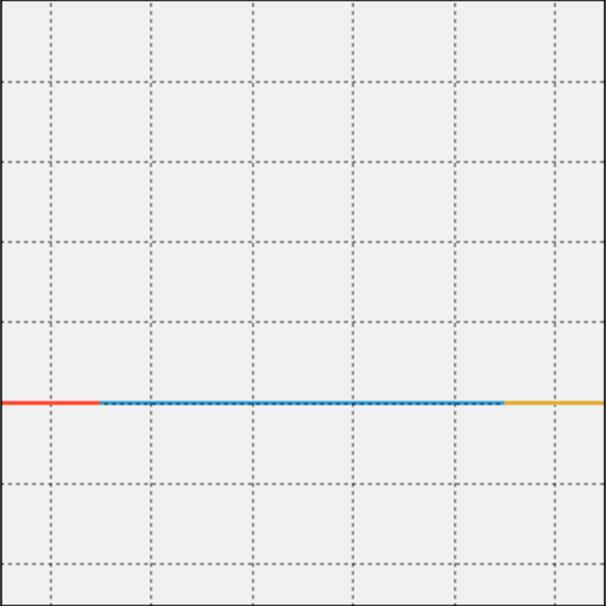
\includegraphics[width=\textwidth]{elastica1}
    \caption{Tom and Jerry}
    \label{fig:TomJerry}   
  \end{subfigure}             
  \begin{subfigure}[b]{0.3\textwidth}
    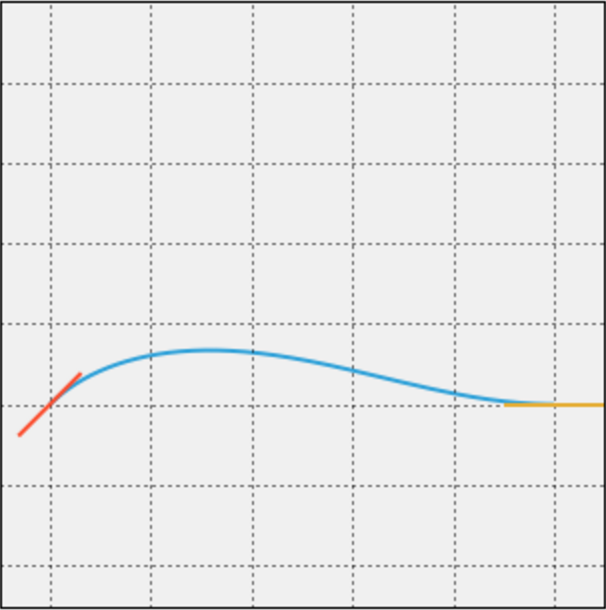
\includegraphics[width=\textwidth]{elastica2}
    \caption{Wall-E}
    \label{fig:WallE}
  \end{subfigure}             
  \begin{subfigure}[b]{0.3\textwidth}
    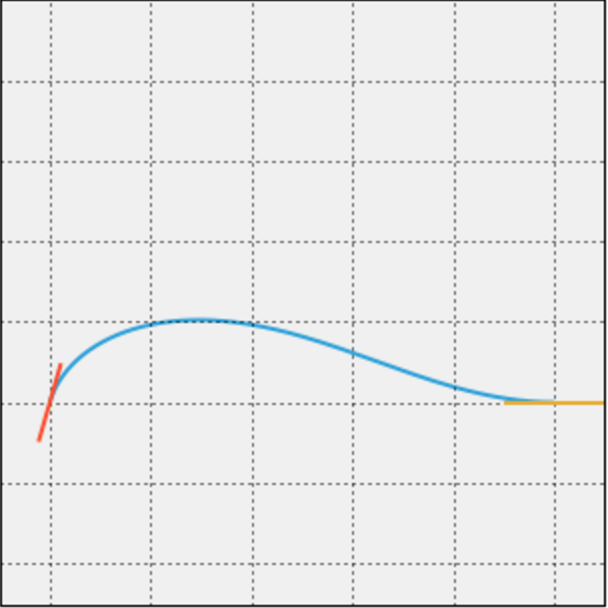
\includegraphics[width=\textwidth]{elastica3}
    \caption{Minions}
    \label{fig:Minnion}
  \end{subfigure}
  \caption{Best Animations}
  \label{fig:animations}
\end{figure}

\begin{figure}[htbp!] 
\centering    
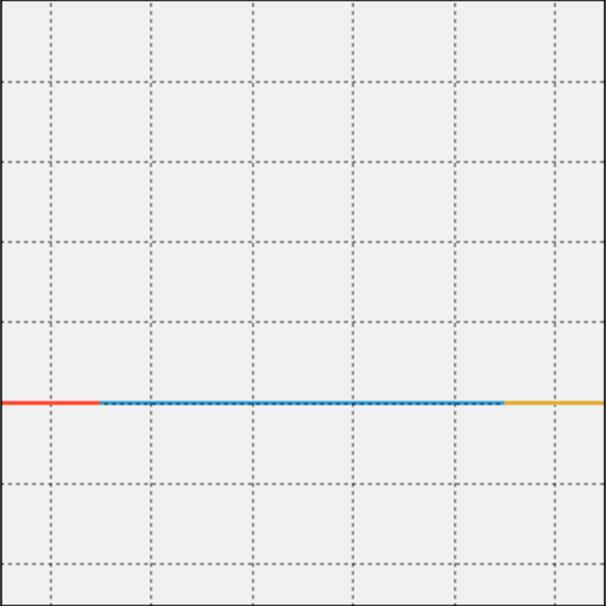
\includegraphics[width=1.0\textwidth]{elastica1}
\caption[Minion]{This is just a long figure caption for the minion in Despicable Me from Pixar}
\label{fig:elastica1}
\end{figure}


\plotfigure{illusion1}{\bt{Visual illusion 1.}The orientations of the small circles inside seem tilted. \cite{baggott2010investigating}}
\plotfigure{illusion2}{\bt{Visual illusion 2.}The lines do not seem parallel, when it reality they are. \cite{vision-computation}}



\chapter{Background}

In explaining the model setup, it is important to first introduce some neuroscience terminology, used in the developed model. As one can imagine the visual cortex is utterly complex. We are focusing on the V1 cortex, analyzing the orientation selective neurons. Even though we are focusing on a specific neurons in only a part of our visual processing pipeline, we make even more simplifications in order to be able to analyze specific features of those neurons. 

\section{Visual field}





Visual field is the area we can see with our eyes. The first few processing steps are illustrated in fig.\ref{visual_fields}. The initial information we receive is changes in light from our retina. This then gets processed by the lateral geniculate nucleus (LGN) and passed down to the Primary visual cortex (V1). V1 receives information about orientation information about the different parts of our visual field. 

\plotfigure{visual_fields}{\bt{Information processing from retina, LGN cells and V1 orientation selective cells.}\cite{receptive-fields}}

Precisely how this information is processed in the main interest of this project. While at a retinal and LGN level, most of the transformations are low-level, V1 starts to extract some patterns useful for the high level visual processing happening in V2, V3, V4, V5 and V6. 

Finally it is also worth mentioning that we see in different details in different parts of our visual fields. Most of the information we perceive is close to the central or foveal vision, which could lead to interesting behavior \cite{knight2008drastically}. However we will ignore this details in our experiments.

\plotfigure{RetinotopicMapping}{\bt{Central and peripheral vision}\cite{retinotopic-mapping} Substantial number of the cells in the retina are devoted to only a small part of our visual field, or central vision. Although relevant to the project, we will ignore this detail, for the benefit of simpler model}

\section{Receptive fields}

In general, a receptive field is defined as a region of the sensory space, which can stimulate a given sensory neuron. In our context we can define the receptive field of a neuron, as the part of visual field, which affects it \cite{Hartline700}. The above two definition are known as classical receptive fields.

It was later discovered that time plays a role as well, making the definition more complicated \cite{deangelis1995receptive}. In our model, described later, we focus on the spatial and ignore the temporal separation of receptive fields. Moreover because neurons are connected to each other, the notion of receptive field can get a bit vague. Because of those connection a neuron, can get excited or inhibited from parts of the visual field, that the neuron is not directly connected to (fig.\ref{F4large}).

To avoid confusion we will stick to the definition of classical receptive fields, and use context modulation for the effects described above.

\plotfigure{F4large}{\bt{Effect of the context on receptive field on a neuron}\cite{cavanaugh2002nature} The firing of neurons is indirectly modulated and their response shifted, based on the stimuli just outside of their receptive field. This leads to some of the complications of explaining receptive field. Even though a certain neuron is tuned for only a certain part of our vision field, for certain orientation, it can be affected by nearby neurons. If we take this to the extreme, then a receptive field is based on all the sensory input we receive.}

\section{Tuning curves}

Different orientation selective neurons are tuned for different orientation at a specific part of the visual field, defined by their receptive field. However they spike not only when the preferred orientation is presented, but also on similar to its preferred orientation. The intensity of spiking, when different orientations are presented, forms a bell shaped curve with a peak the preferred orientation of the neuron. 

\plotfigure{HubelWiesel}{\bt{Tuning curves}\cite{hubel1968receptive} Different orientation bars are presented in a certain part of the visual field(on the left), and the response of the neuron tuned for this specific part of the visual field and $0\degree$. Even though the neuron is tuned for $0\degree$, its spikes when similar orientations are presented. The closer the orientation is to its preferred one, the stronger the response.}


\section{Population coding}

Our final perception of the orientation in a specific part of our visual field is based on the all the spiking of the neurons with that receptive field. Their directions and magnitude form vectors, which when added together give the final perceived orientation.

\plotfigure{populationCoding}{\bt{Population coding in the motor cortex}\cite{amirikian2000directional} Although the above picture illustrates population coding in a different part of the brain, it still illustrates the idea very well. Different orientation selective neurons respond with certain intensity (black bars) and their response are combined to show the final perceived perception(red bars).}  

\chapter{Design}

This paper implements simplified version of visual field, receptive fields, tuning curves and population coding in a recurrent neural network with orientation selective neurons. We start with a simple model with one receptive field, extend the model to multiple receptive fields, define limited and full connectivity and finally implement the elastica principle as well. In this section the different models are described in detail.

The input our model receives is a matrix of numbers from the interval $0-1$, representing different orientation from $0\degree$ to $180\degree$. The output has the same form and represents what orientations the model perceives. Fig.\ref{input_random} shows a nice visualization of a sample input to the model.


\plottwofigures{input_random}{input_structure}{\bt{Visualization of sample input(output) to the model}\\ (A) Random orientations. (B) All orientations from $0\degree$ to $180\degree$, for every $1.8\degree$.}

For every single orientation of the input (every single bar in fig.\ref{input_random}), we have different neurons tuned for different orientations. Fig.\ref{stacked_neurons3} illustrates this. Here it is important two things. 

First of all to detect a specific orientation, we have a stack of different neurons tuned for different orientations (fig.\ref{stacked_neurons3}, (A)). They all spike with different intensities and their collective response, forms the perceived orientation. 

Secondly, every single orientation orientation in our visual field, has its own stack of neurons (fig.\ref{stacked_neurons3}, (B)). Based on all those neurons, we can get accurate information about all the orientations (the higher the number of neurons used, the more accurate the perceived orientation is).

The complexity comes from the fact that the different 'stacks of neurons' are connected with the nearby stacks. 
\plottwofigures{stacked_neurons3}{stacked_neurons2}{\bt{Visualization of the orientation selective neurons and their relationship with the presented input.} (A) Presented orientation(left) and responses of the orientation selective neurons(right). The more saturated the color, the stronger the response is. The neurons will spike with higher intensity, depending on the difference of the presented orientation and their preferred orientations. All the responses are combined, giving the final perceived orientation. (B) Schematic representation of the input and orientation selective neurons. Every orientation bar has its own stack of orientation selective neurons (only the first few are shown).} 

\plottwofiguresS{stacked_neurons}{neuron2}{\bt{Two different visualizations of orientation selective neurons} Orientation selective neurons for a single orientation of our visual field. We use the two pictures interchangeably to explain different concepts.}{.3}

First we implement a visual field with a single orientation. We have a couple of neurons responsible for detecting the orientation (fig.\ref{stacked_neurons}).

As described in \cite{keemink2015unified}, we represent those responses as vectors, with direction their preferred orientation and magnitude, the strength of the response with respect to the stimuli. Summing those vectors gives us the perceived orientation. Although used for recording responses from different types of neurons, fig.\ref{populationCoding} shows how population coding works. Black vectors are neural activity from specific neurons, and the red vector is the sum of all those responses.

Even at this small scale, some experiments (described later) can be run, which show the relation between number of orientation selective neurons used and the accuracy of the perceived orientation.

Next we extend the model so we can feed two orientations and we have orientation selective neurons for the two orientations. We add recurrent connection between the neurons with the same preferred orientations, as showed in fig.\ref{neuron5}, (A), (B). This adds contextual modulation, as the perceived orientation of a single orientation in the visual field is influenced by the other one.

The firing rate of the pairs of same orientation selective neurons in the two visual fields is calculated by the differential equations:

\begin{equation}
\label{model11}
\tau_{syn}\cfrac{dr_{1}(t)}{dt}=-r_{1}(t)+in_{1}+w_{12}r_{2}
\end{equation}


\begin{equation}
\label{model12}
\tau_{syn}\cfrac{dr_{2}(t)}{dt}=-r_{2}(t)+in_{2}+w_{21}r_{1}
\end{equation}

where $\tau_{syn}$ is a constant, $\cfrac{dr_{1/2}(t)}{dt}$ is the change of the firing rate with respect to time, $r_{1/2}(t)$ is the current firing rate, $w_{12/21}$ is the strength between the neurons. $in_{1/2}$ is calculated from the tuning curve of the specific neuron for the  presented orientation. In our model we will use the von Mises function as in \cite{keemink2015unified}. The von Mises function has the following formula:

\eq{A\exp(k\cos(2\alpha_{pref} - \alpha_{actual}))}


The different values of $A$ and $k$ are again described in \cite{keemink2015unified}, but ultimately the function with the correct set of parameters gives us the similarly looking tuning curves as in fig.\ref{HubelWiesel}.


\plottwofigures{neuron5}{neuron3}{\bt{Two orientations, with limited connectivity between neurons}}

Next we extend the model, so we can have any number of orientations (fig.\ref{neuron1}). Every neuron (except the ones at the end at the visual field) is connected with the eight closest neurons, which have the same preferred orientation as his (fig.\ref{neuron1}). We can extend the formulas \ref{model11} and \ref{model12} to:

\begin{equation}
\tau_{syn}\cfrac{dr_{i}(t)}{dt}=-r_{i}(t)+in+\sum_{j} w_{ij}r_{j}
\end{equation}

 
\plotfigureS{neuron1}{\bt{Any number of orientations, with limited connectivity between neurons} *The connections for only one neuron are shown.}{0.7}

The final modification we do, on single neuron level, is to add full connectivity between all the neurons. We set the weights depending on the closeness of the neurons to each other, as well as the similarity of their preferred orientation. To explain how we setup the weights, let use an example. Let's have a $10x10$ visual field with different orientations, as in fig.\ref{input_random} and $9$ orientations selective neurons. Unrolling the $10x10x9$ matrix, we have a vector of $900$ neurons all together. We can setup $900x900$ weight matrix defining the connections between the neurons. 

Having some distance and the orientation constants as $\kappa_{distance}$ and $\kappa_{orientation}$, for every two neurons $l$ and $m$, we model the strength of the connection between them as:

\eq{d=\sqrt{{(i_{l}-i_{m})}^{2}+{{(j_{l}-j_{m})}^{2}}}}

\eq{\delta=min(mod(\alpha_{l}-\alpha_{m},1),mod(\alpha_{m}-\alpha_{l},1))}

\eq{w_{i,j}=w_{j,i}=\kappa_{distance}\cfrac{1}{exp(d)} + \kappa_{orientation}\cfrac{1}{exp(\delta)}}


Based on the above equations we have the updating of the network as:

\begin{equation}
\tau_{syn}\cfrac{dr_{i}(t)}{dt}=-r_{i}(t)+in+\sum_{j=0}^{\#neurons}w_{ij}r_{j}
\end{equation}

We can vectorize our equation (and code), so we have:

\begin{equation}
\tau_{syn}\cfrac{dr_{i}(t)}{dt}=-r_{i}(t)+in+Wr
\end{equation}

The strength of the connection between every two neurons $l$ and $m$ is the same as the recurrent connection between $l$ and $m$, so the matrix is symmetric with respect to the main diagonal. The values along the main diagonals are $0$ (a neuron does not have a connection with itself). We can also notice the general trend of having highest values along the main diagonal and then smaller values the further away we go. This is true for different scales of our matrix - the full matrix (a), the first $100x100$ square (b) as well as the first $10x10$ square (c). The three different scales represent the change in orientation, horizontal and vertical position.



\plotthreefigures{weight1}{weight2}{weight3}{Weight matrix for a full connectivity model. (A) Full weight matrix. (B) First 100 neurons. (C) First 10 neurons. (D) Scale of the values.}

The final part is implementing the elastica principle into the model (still to be done).

\plotfiguresix{elastica1}{elastica2}{elastica3}{elastica4}{elastica5}{elastica6}{\bt{Elastica principle}\\}{.7}




\chapter{Implementation}

(Notes)

Since the model is recursive and changes with respect to time, the output is not only $1$ matrix, but $\cfrac{t}{ts}$ number of matrices, where $t$ is the simulation time and $ts$ is the length of the time step.

(Libraries and Languages Used)

Matlab - http://uk.mathworks.com/products/matlab/

Python 2 - https://www.python.org/download/releases/2.7.2/

Holoviews - http://ioam.github.io/holoviews/

IPython Notebook

(LaTeX)

https://github.com/cfiandra/timeline

\chapter{Timeline}
\begin{figure}
\caption{}
\begin{tikzpicture}[timespan={}]


% timespan={Day} -> now we have days as reference
% timespan={}    -> no label is displayed for the timespan
% default timespan is 'Week'

\timeline[custom interval=true]{May, Jun, Jul, Aug, Sep, Nov, Oct, Dec, Jan, Feb, Mar}
% \timeline[custom interval=true]{3,...,9} -> i.e., from Day 3 to Day 9
% \timeline{8} -> i.e., from Week 1 to Week 8


% put here the phases
\begin{phases}
\initialphase{involvement degree=4.75cm,phase color=black}
\phase{between week=5 and 7 in 0.7,involvement degree=4cm, phase color=black}
\phase{between week=7 and 9 in 0.7,involvement degree=2cm, phase color=black}
\phase{between week=5 and 9 in 0.7,involvement degree=4cm, phase color=green}
\phase{between week=9 and 11 in 0.1,involvement degree=2.25cm}
\phase{between week=8 and 11 in 0.7,involvement degree=2.25cm ,phase color=blue!80!cyan}
\end{phases}

% put here the milestones
\addmilestone{at=phase-0.180,direction=90:1cm,text={Project allocation},text options={above}}
\addmilestone{at=phase-0.270,direction=270:1cm,text={Sensory Systems (MIT OpenCourseWare)},text options={below}}

\addmilestone{at=phase-1.130,direction=130:2cm,text={Literature review},text options={above}}
\addmilestone{at=phase-1.230,direction=230:1cm,text={Neural Computation},text options={below}}
\addmilestone{at=phase-1.290,direction=290:2cm,text={Machine Learning Practical},text options={below}}

\addmilestone{at=phase-2.100,direction=100:3cm,text={More literature review},text options={above}}
\addmilestone{at=phase-2.310,direction=310:3cm,text={Neural Information Processing},text options={below}}

\addmilestone{at=phase-3.170,direction=170:1cm,text={Started working on Matlab implementation},text options={above}}
\addmilestone{at=phase-3.140,direction=140:1cm,text={Visual fields},text options={above}}
\addmilestone{at=phase-3.120,direction=120:1cm,text={Tuning curves},text options={above}}
\addmilestone{at=phase-3.90,direction=90:1cm,text={Population coding},text options={above}}
\addmilestone{at=phase-3.60,direction=60:1cm,text={Simple Dynamics},text options={above}}
\addmilestone{at=phase-3.30,direction=30:1.5cm,text={Dynamics with weight matrix},text options={above}}
\addmilestone{at=phase-3.270,direction=270:0.5cm,text={Python implementation},text options={below}}
\addmilestone{at=phase-3.300,direction=300:0.5cm,text={Elastica principle},text options={below}}

\addmilestone{at=phase-4.120,direction=120:0.3cm,text={Matlab experiments},text options={above}}
\addmilestone{at=phase-4.310,direction=310:0.3cm,text={Python experiments},text options={below}}

\addmilestone{at=phase-5.140,direction=140:0.34cm,text={Interim report},text options={above}}
\addmilestone{at=phase-5.50,direction=50:0.34cm,text={Write},text options={above}}
\addmilestone{at=phase-5.330,direction=330:0.34cm,text={Write},text options={below}}
\addmilestone{at=phase-5.20,direction=20:1cm,text={Final write up},text options={above}}

\end{tikzpicture}
\label{timeline}
\floatfoot{\bt{Timeline of the project}\\\textcolor{gray}{Research}\\\textcolor{green}{Implementation}\\\textcolor{yellow}{Experiments}\\\textcolor{blue}{Write up}}
\end{figure}

Fig.\ref{timeline} illustrates the work I have done so far and my plan until end of march, when the final deadline for the report is. After the project was allocated to me, I spend some time during the summer watching online courses on neuroscience and sensory systems.

Beginning of the year, I took Neural Computation to get even more background. I started implementing all the necessary parts, in order to simulate the model - visual fields, tuning curves, population coding, etc. Afterwards I started implementing dynamics in the system, gradually extending the model. In my final model, I assume full connectivity between all the neurons. The connection at first are modeled based on the distance and difference in preferred orientations between them. My next goal is to incorporate the elastica principle into my model. 

At first I opted to use Matlab, as I had some experience with it. However with time, as I added some complexity to my model, I realized Matlab is not the base choice for the project. I decided to switch to Python, using Notebooks and Holoviews. Notebooks are a lot better way for structuring the code and write up at the same time. Holoviews was the other main reason, as it provides advanced plotting capabilities on multidimensional data, which is really viable when visualizing the output of recurrent neural networks for different time steps.



\chapter{Evaluation}

\chapter{Conclusions}

% use the following and \cite{} as above if you use BibTeX
% otherwise generate bibtem entries
\bibliographystyle{plain}
\bibliography{mybib}

\end{document}
